% hfg_ramification_disjointness.tex
% Standalone TikZ figure: ramification-disjointness argument for the
% four-field Galois closure (CLAIMS_REGISTER.md entry 15).
% Compile with: pdflatex hfg_ramification_disjointness.tex
\documentclass[tikz,border=8pt]{standalone}
\usepackage{amsmath,amssymb}
\usetikzlibrary{arrows.meta,positioning}

\definecolor{hfggreen}{HTML}{2A5E2A}
\definecolor{hfgtan}{HTML}{7B5A2E}
\definecolor{hfgbg}{HTML}{F7F4EF}

\begin{document}
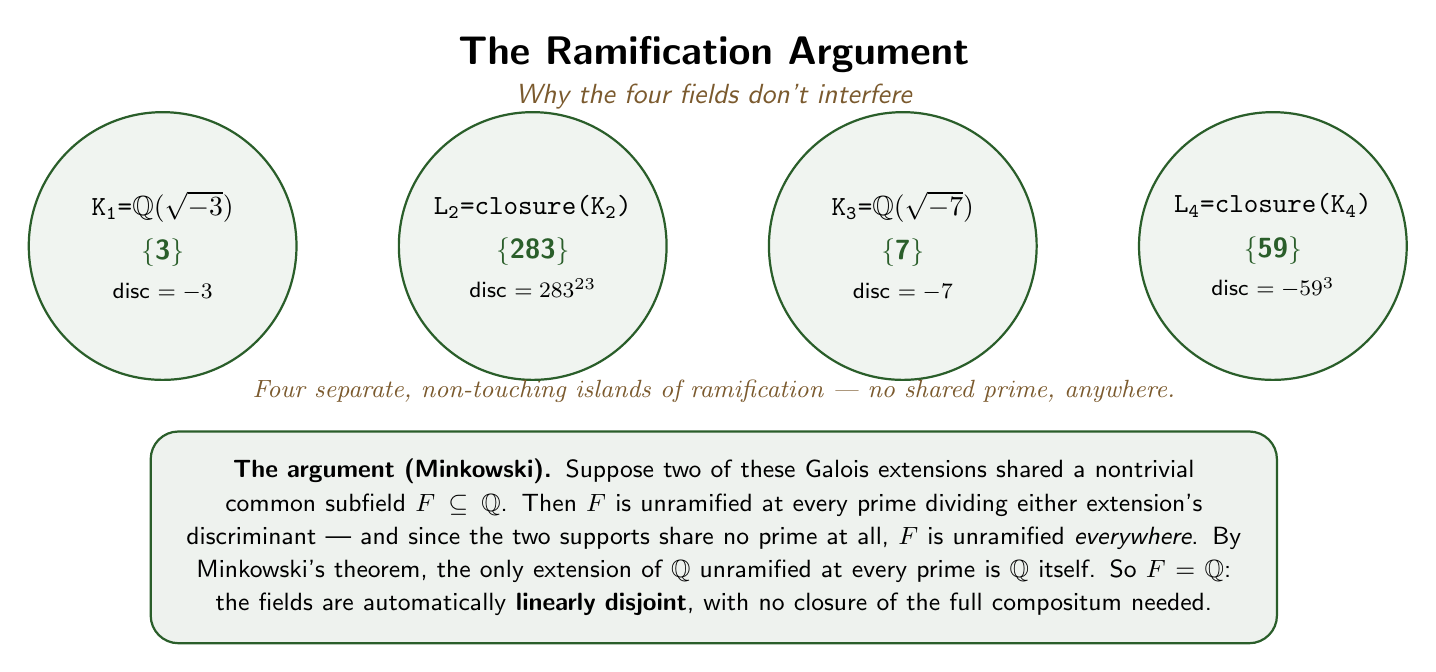
\begin{tikzpicture}[
  font=\sffamily,
  island/.style={circle, draw=hfggreen, fill=hfggreen!7, minimum size=3.4cm, align=center, thick},
  card/.style={rounded corners=10pt, draw=hfggreen, fill=hfggreen!8, thick, align=center},
  interp/.style={rounded corners=10pt, draw=hfgtan, fill=hfgtan!8, thick, align=center},
  arr/.style={-{Latex[length=3mm]}, hfggreen, thick}
]

\node[align=center] at (7,7.6) {\Large\bfseries The Ramification Argument\\[2pt]
  \normalsize\itshape\color{hfgtan} Why the four fields don't interfere};

% Four disjoint islands
\node[island] (K1) at (0,5.4)  {\texttt{K\textsubscript{1}=$\mathbb{Q}(\sqrt{-3})$}\\[4pt]{\bfseries\color{hfggreen}\{3\}}\\[2pt]\footnotesize disc $=-3$};
\node[island] (L2) at (4.7,5.4) {\texttt{L\textsubscript{2}=closure(K\textsubscript{2})}\\[4pt]{\bfseries\color{hfggreen}\{283\}}\\[2pt]\footnotesize disc $=283^{23}$};
\node[island] (K3) at (9.4,5.4) {\texttt{K\textsubscript{3}=$\mathbb{Q}(\sqrt{-7})$}\\[4pt]{\bfseries\color{hfggreen}\{7\}}\\[2pt]\footnotesize disc $=-7$};
\node[island] (L4) at (14.1,5.4){\texttt{L\textsubscript{4}=closure(K\textsubscript{4})}\\[4pt]{\bfseries\color{hfggreen}\{59\}}\\[2pt]\footnotesize disc $=-59^{3}$};

\node[align=center, hfgtan, font=\itshape\small] at (7,3.55)
  {Four separate, non-touching islands of ramification --- no shared prime, anywhere.};

% Minkowski box
\node[card, text width=13.6cm, inner sep=10pt] (mink) at (7,1.7) {
  \small
  \textbf{The argument (Minkowski).} Suppose two of these Galois extensions shared a
  nontrivial common subfield $F \subseteq \mathbb{Q}$. Then $F$ is unramified at every
  prime dividing either extension's discriminant --- and since the two supports share
  no prime at all, $F$ is unramified \emph{everywhere}. By Minkowski's theorem, the only
  extension of $\mathbb{Q}$ unramified at every prime is $\mathbb{Q}$ itself. So $F=\mathbb{Q}$:
  the fields are automatically \textbf{linearly disjoint}, with no closure of the full
  compositum needed.
};

\end{tikzpicture}
\end{document}
